\setcounter{section}{2}

\Needspace{5\baselineskip}
\hypertarget{transformer}{%
\section{Transformer}\label{transformer}}

Transformer是Google于2017年提出的架构，是目前所有大模型架构的基础。

\begin{figure}[htbp]
\centering
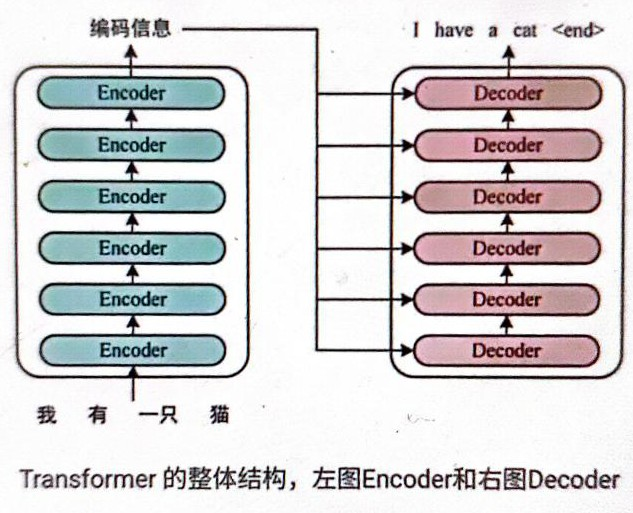
\includegraphics{images/image-0016.jpeg}
\caption{Transformer 的整体结构示意图}
\end{figure}

Transformer 的整体结构：左侧为 Encoder，右侧为 Decoder。

\begin{figure}[htbp]
\centering
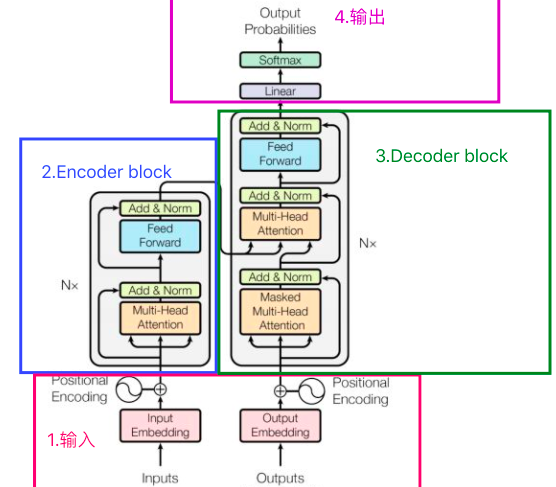
\includegraphics{images/image-0017.png}
\caption{Transformer 模块总览图}
\end{figure}

\Needspace{5\baselineskip}
\hypertarget{ux4e00ux8f93ux5165}{%
\subsection{一、输入}\label{ux4e00ux8f93ux5165}}

\begin{enumerate}
\def\labelenumi{\arabic{enumi}.}
\item
  左下 inputs 表示输入序列，右下 Outputs (shifted right) 表示输出内容（其实是只提供该时间步以前生成的内容，训练预测能力）。
\item
  词嵌入 (Word Embedding)：每个词会被映射到一个固定长度的向量。例如，``猫''可能被表示为 \texttt{{[}0.1,\ -0.4,\ 0.8,\ ...{]}}。这些向量在训练开始时是随机的，模型会逐渐学习到让意思相近的词（如``猫''和``虎''）拥有更相似的向量。
\item
  位置编码 (Positional Encoding)：由于 Transformer 抛弃了 RNN 的顺序结构，后续的编码器本身无法感知词语的位置。没有位置信息，``我打你''和``你打我''在模型看来是一样的。为了解决这个问题，我们需要给每个词的向量中加入``位置信号''。后面会介绍位置编码。
\end{enumerate}

\Needspace{5\baselineskip}
\hypertarget{ux4e8cencoder-block}{%
\subsection{二、Encoder Block}\label{ux4e8cencoder-block}}

\begin{enumerate}
\def\labelenumi{\arabic{enumi}.}
\item
  多头自注意力 (Multi-Head Attention)：编码器的核心，读取输入内容，通过多头自注意力机制，逐层得到富含上下文信息的中间表示。
\item
  Add：参照了残差神经网络，与输入直接相加。
\item
\Needspace{5\baselineskip}
  Layer Normalization：对上一步的结果进行归一化处理。它能使模型训练过程更加稳定和快速，减少对参数初始化的敏感度。我们用 Layer Normalization (LN)，而不是 Batch Normalization (BN)，这二者的区别是：
\end{enumerate}

假设我们的输入数据形状为 {[}Batch\_Size, Seq\_Len, d\_model{]}，比如：{[}32, 10, 512{]}（32个句子，每句10个词，每个词512维）。

Batch Normalization (BN) 是``纵向切''，它固定特征维度，统计整个Batch的均值和方差。对于第i个特征维度（比如第0维），它会把这32个句子中、所有位置的词的第0维拿出来求平均。这在NLP中非常糟糕。因为不同句子的长度不同（通常靠Padding补齐），且不同位置的词语义差异极大，不同语段中各个特征维度的分布也往往有天然差异，强行让所有词语的第0维符合正态分布是不合理的，相当于``扭曲''了embedding空间，改变了向量之间的相似度，直接破坏embedding空间中存储的语义信息。

Layer Normalization (LN)是``横向切''，它固定样本（Token），统计该Token自身所有维度的均值和方差。对于第1个句子的第1个词（一个512维的向量），它计算这 512 个数值的均值和方差，然后进行伸缩，实质上抹平了向量模长的差异，让每个token的各个特征近似服从N(0,1)，这样点积就可以近似表示余弦相似度，即语义相似度。LN 将所有向量拉回到同一个``单位球壳''附近，让模型专注于学习方向（特征的组合方式，即语义），而不是数值的大小。

\begin{enumerate}
\def\labelenumi{\arabic{enumi}.}
\setcounter{enumi}{3}
\tightlist
\item
  Feed Forward：在每个注意力层之后，编码器和解码器都会有一个简单的前馈神经网络。这个网络对每个位置的向量独立地进行一次非线性变换。它由两个线性层和一个 ReLU 激活函数组成，可以看作是对注意力机制提取出的信息进行进一步的加工和提炼，增加模型的非线性能力。
\end{enumerate}

\Needspace{5\baselineskip}
\hypertarget{ux4e09decoder-block}{%
\subsection{三、Decoder Block}\label{ux4e09decoder-block}}

\Needspace{4\baselineskip}
\begin{enumerate}
\def\labelenumi{\arabic{enumi}.}
\tightlist
\item
  带掩码的多头自注意力 (Masked Multi-Head Self-Attention)
\end{enumerate}

（1）目的与工作方式：``回顾已写内容''。在生成下一个词时，解码器需要知道自己前面已经写了什么，以保证句子的连贯性。例如，已经写了 ``I am a''，下一个词很可能是 ``cat''，而不是重复生成 ``I''。它和编码器中的自注意力机制几乎完全一样，都是为了计算序列内部词与词之间的关系。

（2）为什么需要掩码？

在训练时，我们已经知道了完整的译文（例如 ``I am a cat''）。如果没有掩码，当模型在预测 ``am'' 这个词时，它会``偷看''到后面的 ``a'' 和 ``cat''，这显然是在作弊，模型学不到真正的预测能力。

（3）如何实现掩码？

掩码是一个``上三角矩阵''，它在计算注意力分数后、进行 Softmax 之前起作用。它会强制将所有未来位置 \((i,j)\)（\(i>j\)）的注意力分数，即 \(q_i\) 与 \(k_j\) 的点积设置为一个绝对值极大的负数（例如 \(-10^9\)）。

效果：绝对值极大的负数经过 Softmax 函数后，其对应的权重会无限接近于0。这样一来，模型在计算任意位置的输出时，其注意力权重只能分布在当前位置和之前的位置上，从而保证了模型无法``看到未来''。

\Needspace{4\baselineskip}
\begin{enumerate}
\def\labelenumi{\arabic{enumi}.}
\setcounter{enumi}{1}
\tightlist
\item
  编码器-解码器注意力 (Encoder-Decoder Attention / Cross-Attention)
\end{enumerate}

（1）目的：这是连接编码器和解码器的核心桥梁。它让解码器在生成译文的每一步，都能去关注原文中最相关的部分。它用自己当前的理解(Q)去查询原文的完整信息 (K和V)，看看原文的哪一部分对生成下一个词最重要。

\Needspace{8\baselineskip}
\Needspace{5\baselineskip}
（2）工作方式：这也是一个多头注意力层，但它的 \(Q,K,V\) 来源不同：

查询向量 (Query, Q)：来自解码器前一个子层（即带掩码的自注意力层）的输出。这个 Q 向量代表了``写作部''当前的需求，可以理解为：``根据我已经写出的内容（比如 `I am'），我现在需要什么信息来决定下一个词？''

键向量 (Key, K) 和 值向量 (Value, V)：全部来自编码器栈的最终输出（即``理解部''的最终版精读笔记）。这两个向量代表了原文的完整信息，并且在解码的整个过程中是固定不变的。

（3）比喻：解码器（作者）拿着自己的草稿（Q 向量）去问编码器（原文摘要）：``我的草稿写到这了，请问你原文中哪部分内容跟我现在要写的最相关？'' 编码器通过 K, V 向量回答它，解码器据此获得生成下一个词的关键线索。例如，当解码器生成到与 ``猫'' 对应的位置时，这一层的注意力会高度集中在编码器输出中代表 ``猫'' 的那个向量上。

\Needspace{4\baselineskip}
\begin{enumerate}
\def\labelenumi{\arabic{enumi}.}
\setcounter{enumi}{2}
\tightlist
\item
  前馈神经网络 (Position-wise Feed-Forward Network)
\end{enumerate}

（1）目的：``消化整合，深入思考''。

（2）工作方式：这个子层与编码器中的前馈网络完全相同。它接收来自编码器-解码器注意力层的输出向量，并对其进行一次非线性变换。

（3）比喻：在回顾了自己写的内容（Masked Self-Attention）并查阅了原文（Encoder-Decoder Attention）之后，解码器需要一个``独立思考''的过程，将这些信息进行整合、加工和提炼，最终形成一个准备用于预测下一个词的、信息高度浓缩的向量。这个``独立思考''的过程就是由前馈网络完成的。

\Needspace{5\baselineskip}
\hypertarget{ux56dbux8f93ux51fa}{%
\subsection{四、输出}\label{ux56dbux8f93ux51fa}}

\begin{enumerate}
\def\labelenumi{\arabic{enumi}.}
\tightlist
\item
  取注意力层输出矩阵的什么内容？
\end{enumerate}

注意力层输出矩阵的形状为 \texttt{{[}seq\_len,d\_model{]}}，其中 \texttt{seq\_len} 是输入序列长度。

我们的目标是预测序列的 Next Token（如第4个词），我们只需要关注序列中最后一个 Token（第3个词）经过模型处理后的输出向量。因为在 Masked Self-Attention（带掩码的自注意力）机制下，最后一个 Token 的向量 \(h\) 已经聚合了整个序列的所有历史信息。

若希望得到原序列经过交互后富含上下文信息的序列：输出整个矩阵对应的Token序列。

\Needspace{4\baselineskip}
\begin{enumerate}
\def\labelenumi{\arabic{enumi}.}
\setcounter{enumi}{1}
\tightlist
\item
  计算相似度
\end{enumerate}

得到输出向量后，我们会将其转化为输出 Token，具体操作为：和词表中所有 Token 计算点积相似度，这一步可以用矩阵乘法表示为 \(hW\)（\(W\) 是输出层的权重矩阵，每一行被视为词表中对应词的嵌入向量），经过 Softmax 后输出。

\Needspace{5\baselineskip}
为什么可以用点积作为相似度呢？我们先从余弦相似度说起：

假设我们有两张不同的猫的图片，对应向量 \(x\) 和 \(y\)，我们希望它们的欧氏距离很小。在少数轮廓、皮毛之类的信号维度上，\(x_i\) 和 \(y_i\) 的值可能很相似，所以 \((x_i-y_i)^2\) 很小；但在草地、光照、拍摄角度等海量噪音维度上，\(x_i\) 和 \(y_i\) 会有微小的随机差异，每个 \((x_i-y_i)^2\) 可能不大，但它们的数量是压倒性的。

\Needspace{5\baselineskip}
欧氏距离的 \(L_2\) 度量本质上是一个无差别的累加器：

\[
d^2(x,y)=\sum_{i\in\text{Signal}}(x_i-y_i)^2+\sum_{j\in\text{Noise}}(x_j-y_j)^2
\]

它将信号维度上的微小差异与海量噪音维度上的随机差异同等对待，并将它们的平方和累加起来。最终总距离的计算结果可能由噪音项的总和主导，因此并不适合作为高维语义向量的主要相似度度量。

\Needspace{5\baselineskip}
余弦相似度衡量的是两个向量在方向上的接近程度，直接忽略它们的绝对长度：

\[
d_{\cos}(x,y)=\frac{x\cdot y}{\|x\|\|y\|}=\frac{\sum_{i=1}^{D}x_i y_i}{\sqrt{\sum_{i=1}^{D}x_i^2}\sqrt{\sum_{i=1}^{D}y_i^2}}
\]

\Needspace{5\baselineskip}
方向是一种比长度更稳健的度量，承载了更纯净的各向异性信号：

\begin{itemize}
\tightlist
\item
  高维中随机的背景噪音几乎都是正交的，点积会非常接近 0。
\item
  而构成猫的信号维度在不同猫图片向量中表现出一致的方向性，点积可以增强这一点。
\end{itemize}

\Needspace{5\baselineskip}
实际上，大模型中使用的多为点积相似度。原因：

（1）效率与简化计算\hspace{0pt}：点积运算 (A · B) 本身比余弦相似度计算（需要先计算点积，再除以两个向量的模长 \textbar\textbar A\textbar\textbar{} * \textbar\textbar B\textbar\textbar）更简单高效。在自回归生成中，模型需要为词表中的每一个词（通常是数万甚至数十万个）计算一个相似度分数，点积能显著减少计算量。

（2）与Softmax的天然配合：模型的学习过程已经内化了对向量``长度''的调整，各个向量长度几乎差不多。这时，点积计算得到的分数（通常称为 logits）会直接输入到 Softmax 函数中，以转换为下一个词的概率分布。所有词都除以模长或者都不除以模长对于经过 Softmax 函数后的概率分布没有影响，因此这一步可以被省略而不影响模型性能。

\Needspace{4\baselineskip}
\begin{enumerate}
\def\labelenumi{\arabic{enumi}.}
\setcounter{enumi}{2}
\tightlist
\item
  自回归输出
\end{enumerate}

模型每次利用序列前文 \([x_1,\ldots,x_{i-1}]\) 作为输入，输出一个 token 即 \(x_i\)，再将 \([x_1,\ldots,x_i]\) 作为新的输入，以此类推。这个``输入 -\textgreater{} 解码器栈处理 -\textgreater{} 线性层 -\textgreater{} Softmax -\textgreater{} 选择词语''的循环会一直进行下去，直到选出的词是特殊的句子结束符 \texttt{\textless{}/s\textgreater{}} 为止。这个过程是串行的。

\FloatBarrier
\Needspace{5\baselineskip}
\hypertarget{ux53c2ux8003ux6587ux732e-69}{%
\subsection{参考文献}\label{ux53c2ux8003ux6587ux732e-69}}

\vspace{0.25em}
\begin{itemize}
\tightlist
\item
  Vaswani, A., Shazeer, N., Parmar, N., et al.~(2017). \href{https://arxiv.org/abs/1706.03762}{Attention Is All You Need}. NeurIPS 2017.
\end{itemize}

\clearpage
